\chapter{Исследовательская часть}
\section{Характеристики устройства}

Исследования проводились на машине со следующими характеристиками:
\begin{itemize}[label=---]
	\item процессор Intel(R) Core(TM) i5-10210U, тактовая частота 1.60 ГГц;
	\item оперативная память: 16 ГБ;
	\item операционная система: Ubuntu 22.04.4 LTS.
\end{itemize}

\section{Параметризация}

Для муравьиного алгоритма была произведена параметризация для определения наиболее оптимальных, в смысле минимизации ошибки ответа алгоритма по сравнению с точным значением, значений параметров:
\begin{itemize}
	\item $\alpha$~---~параметр, определяющий <<жадность>> решения;
	\item $\beta = 1 - \alpha$~---~параметр, определяющий <<стадность>> решения;
	\item $\rho$~---~коэффициент испарения феромона;
	\item $e$~---~число элитных муравьев.
\end{itemize}

Параметризация проводилась с использованием полных неориентированных графов из 10 вершин, привязанных к карте местности Африки, для поиска незамкнутого маршрута. Пример графа приведен на рисунке~\ref{fig:graph}.

\begin{figure}[H]
	\centering
	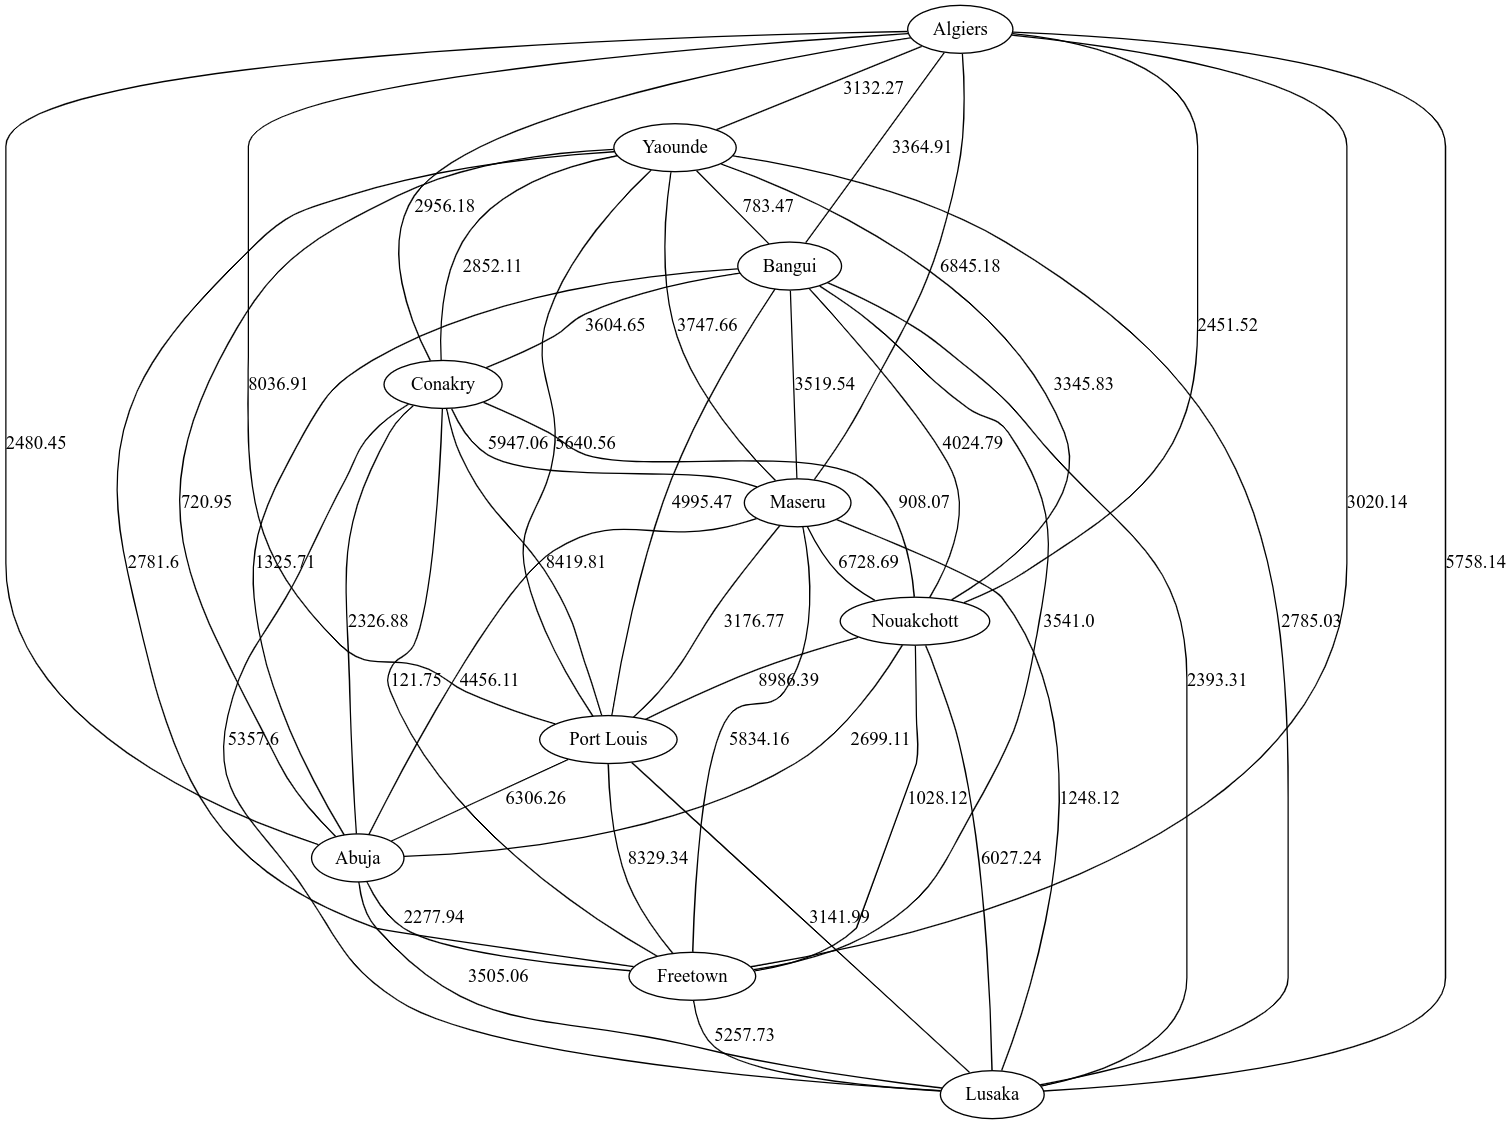
\includegraphics[width=\textwidth]{graph.png}
	\caption{Пример графа для параметризации}
	\label{fig:graph}
\end{figure}

Матрицы смежности для графов, на которых производилась параметризация:
\begin{itemize}
	\item граф 1:
	$$
	\begin{pmatrix}
		0 & 8986.4 & 2451.5 & 3345.8 & 2699.1 & 4024.8 & 1028.1 & 6027.2 & 908.1 & 6728.7\\
		8986.4 & 0 & 8036.9 & 5640.6 & 6306.3 & 4995.5 & 8329.3 & 3142.0 & 8419.8 & 3176.8\\
		2451.5 & 8036.9 & 0 & 3132.3 & 2480.5 & 3364.9 & 3020.1 & 5758.1 & 2956.2 & 6845.2\\
		3345.8 & 5640.6 & 3132.3 & 0 & 720.9 & 783.5 & 2781.6 & 2785.0 & 2852.1 & 3747.7\\
		2699.1 & 6306.3 & 2480.5 & 720.9 & 0 & 1325.7 & 2277.9 & 3505.1 & 2326.9 & 4456.1\\
		4024.8 & 4995.5 & 3364.9 & 783.5 & 1325.7 & 0 & 3541.0 & 2393.3 & 3604.7 & 3519.5\\
		1028.1 & 8329.3 & 3020.1 & 2781.6 & 2277.9 & 3541.0 & 0 & 5257.7 & 121.7 & 5834.2\\
		6027.2 & 3142.0 & 5758.1 & 2785.0 & 3505.1 & 2393.3 & 5257.7 & 0 & 5357.6 & 1248.1\\
		908.1 & 8419.8 & 2956.2 & 2852.1 & 2326.9 & 3604.7 & 121.7 & 5357.6 & 0 & 5947.1\\
		6728.7 & 3176.8 & 6845.2 & 3747.7 & 4456.1 & 3519.5 & 5834.2 & 1248.1 & 5947.1 & 0\\
	\end{pmatrix}
	$$
	\item граф 2:
	$$
	\begin{pmatrix}
		0 & 8986.4 & 1626.0 & 1655.4 & 2242.1 & 5979.2 & 465.4 & 6405.7 & 7972.6 & 6448.0\\
		8986.4 & 0 & 8740.2 & 7337.7 & 6769.7 & 3728.3 & 8867.0 & 2807.2 & 1062.8 & 2604.1\\
		1626.0 & 8740.2 & 0 & 1983.9 & 2708.1 & 5250.7 & 2056.5 & 6556.7 & 7843.7 & 6455.1\\
		1655.4 & 7337.7 & 1983.9 & 0 & 731.3 & 4412.8 & 1637.0 & 4826.3 & 6335.1 & 4827.4\\
		2242.1 & 6769.7 & 2708.1 & 731.3 & 0 & 4146.9 & 2099.2 & 4166.7 & 5741.7 & 4208.9\\
		5979.2 & 3728.3 & 5250.7 & 4412.8 & 4146.9 & 0 & 6044.9 & 3006.1 & 3140.4 & 2561.5\\
		465.4 & 8867.0 & 2056.5 & 1637.0 & 2099.2 & 6044.9 & 0 & 6211.2 & 7832.7 & 6291.9\\
		6405.7 & 2807.2 & 6556.7 & 4826.3 & 4166.7 & 3006.1 & 6211.2 & 0 & 1749.5 & 481.7\\
		7972.6 & 1062.8 & 7843.7 & 6335.1 & 5741.7 & 3140.4 & 7832.7 & 1749.5 & 0 & 1548.1\\
		6448.0 & 2604.1 & 6455.1 & 4827.4 & 4208.9 & 2561.5 & 6291.9 & 481.7 & 1548.1 & 0\\
	\end{pmatrix}
	$$
	\item граф 3:
	$$
	\begin{pmatrix}
		0 & 8986.4 & 5477.6 & 8203.4 & 4188.2 & 4951.6 & 5979.2 & 2154.7 & 6405.7 & 628.8\\
		8986.4 & 0 & 3543.3 & 1618.5 & 4863.2 & 5812.3 & 3728.3 & 6883.9 & 2807.2 & 8701.8\\
		5477.6 & 3543.3 & 0 & 2834.2 & 1658.3 & 3175.9 & 1544.1 & 3461.7 & 1680.4 & 5262.4\\
		8203.4 & 1618.5 & 2834.2 & 0 & 4449.5 & 4339.2 & 2386.5 & 6281.7 & 2995.5 & 8056.9\\
		4188.2 & 4863.2 & 1658.3 & 4449.5 & 0 & 3839.9 & 2984.8 & 2040.4 & 2223.3 & 3846.4\\
		4951.6 & 5812.3 & 3175.9 & 4339.2 & 3839.9 & 0 & 2118.5 & 4073.2 & 4850.3 & 5159.4\\
		5979.2 & 3728.3 & 1544.1 & 2386.5 & 2984.8 & 2118.5 & 0 & 4310.1 & 3006.1 & 5941.2\\
		2154.7 & 6883.9 & 3461.7 & 6281.7 & 2040.4 & 4073.2 & 4310.1 & 0 & 4251.8 & 1819.0\\
		6405.7 & 2807.2 & 1680.4 & 2995.5 & 2223.3 & 4850.3 & 3006.1 & 4251.8 & 0 & 6030.9\\
		628.8 & 8701.8 & 5262.4 & 8056.9 & 3846.4 & 5159.4 & 5941.2 & 1819.0 & 6030.9 & 0\\
	\end{pmatrix}
	$$
\end{itemize}

Результаты параметризации представлены в приложении A.

\subsection{Замеры времени}

Замеры производились с использованием полных графов с числом вершин от 2 до 11. Параметры муравьиного алгоритма: $\alpha=0.1$, $\beta = 0.9$, число дней $= 100$, $\rho=0.1$, число элитных муравьев $= 4$. Полученные зависимости представлены на рисунке~\ref{fig:plot}.
\begin{figure}[H]
	\centering
	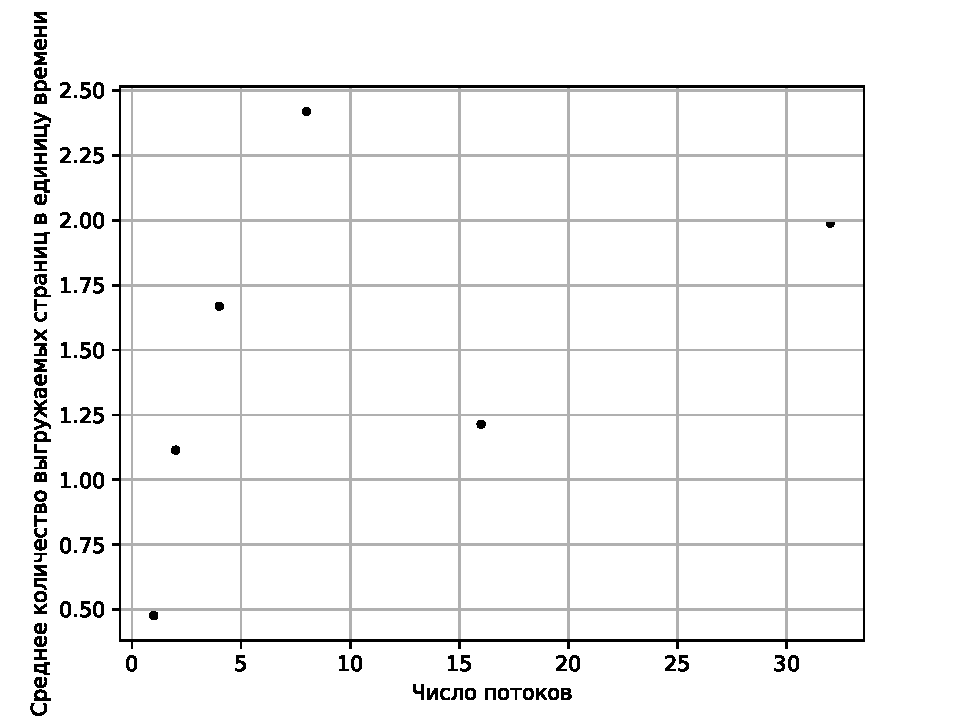
\includegraphics[width=\textwidth]{plot.pdf}
	\caption{Графики зависимости времени решения задачи коммивояжера от числа вершин в графе}
	\label{fig:plot}
\end{figure}

\section{Вывод}

В результате параметризации были определены следующие оптимальные параметры муравьиного алгоритма:
\begin{itemize}
	\item $\alpha \in [0,\ 0.4]$;
	\item $\beta \in [0.6,\ 0.1]$;
	\item $\rho \in [0.1,\ 0.2]$;
	\item $\text{число дней} > 100$;
	\item $\text{число элитных муравьев} \in [5, 15]$.
\end{itemize}

По результатам замеров времени выполнения было выявлено, что муравьиный алгоритм начинает превосходить в скорости выполнения полный перебор, для графов с числом вершин не менее 9.

\clearpage